\documentclass{handout_utfpr}

\usepackage{xspace}
\usepackage{pbox}
\usepackage[brazil]{babel}
\usepackage{xcolor}
\usepackage[alf]{abntex2cite}
\usepackage{url}
\definecolor{dark-gray}{gray}{0.20}
\definecolor{light-gray}{gray}{0.85}

\newcommand{\com}[1]{
\colorbox{light-gray}{\texttt{\pbox{\textwidth}{\$ #1}}}
}

\newcommand{\cominline}[1]{
\colorbox{light-gray}{\texttt{\pbox{\textwidth}{#1}}}
}

\subjnum{CC31C}
\subject{Introdução à Ciência da Computação}
\subjelab{Introdução ao \LaTeX}

\handoutdate{\today}

\begin{document}
\maketitle

\input{contents/intro} %Introdução a typesetting

\section{WYSIWYG}

A maioria dos softwares responsáveis por processamento de palavras utilizam uma interface que permite que o usuário veja algo muito similar ao resultado final enquanto o documento está sendo criado. Essa interface pode ser chamada de WYSIWYG (``What You See Is What You Get'', ou em uma tradução literal, ``O que você vê é o que você obtém''). Um exemplo de programa que se encaixa nesta classificação é o \textbf{MS Word}.

Em editores WYSIWYG, pedaços de códigos são inseridos no documento para indicar onde a fonte deve mudar de tamanho, onde usar itálico, ou negrito, etc. Esses pedaços de código não são vistos pelo usuário em momento algum, portanto só é possível editar esse arquivo utilizando o próprio software que o criou. Com o \LaTeX, o documento consiste de apenas um arquivo de texto, que pode ser modificado com qualquer editor. É possível dizer, então, que WYSIWYW (``What You See Is What You Want'', ou ``O que você vê é o que você quer'').

\subsection{\LaTeX\ vs WYSIWYG}%Por que o \LaTeX é melhor que softwares WYSIWYG?} 
Embora existam diversas situações onde a utilização de um programa é preferida à de outro por inúmeras razões, existem alguns motivos que podem servir como motivação na escolha do \LaTeX\ como sua ferramenta para criação de textos.

\begin{itemize}
\item Velocidade.

Qualquer ação que requer um mouse ou cliques para acesso de menus será mais lento do que digitar algumas teclas do teclado. Isso significa que digitar caracteres especiais, como uma letra grega, ou principalmente funções serão muito mais rápidos no \LaTeX.

Na edição de arquivos muito grandes, e com muitas figuras e equações, o MS Word, por exemplo, se torna muito mais lerdo, já que ações como mover a barra de rolagem de arquivos pesados requerem muito do processador e da memória. Editar um simples arquivo de texto já não causa tantos problemas para a máquina e a modificação pode ser feita rapidamente.

\item Segurança.

Os arquivos dos editores comuns são armazenados em uma forma binária. Se este arquivo for corrompido por qualquer motivo, o usuário pode perder muitas horas de trabalho. Com arquivos de texto, como no \LaTeX, se um editor falhar, basta abrir o arquivo em outro.

\item Separação de conteúdo e formatação.

A separação em seções e subseções de texto no \LaTeX\ torna muito mais fácil para o escritor se concentrar no texto e na sua ordem de apresentação do que em detalhes superficiais como tamanhos de fonte e estilos.

\item Integração com Sistema de Controle de Versões.

  O \LaTeX\ propicia o uso de sistemas de controles de versão, já que seu formato em texto puro pode ser gerenciado de forma simples por estes sistemas. Desta forma a cooperação entre múltiplos usuários durante a escrita de um texto se torna mais fácil.

  %que precisam integrar o seu projeto em um só, o \LaTeX\ se torna essencial simplesmente pelo seu texto simples, dessa forma também armazenando pouco espaço no servidor. A comparação de dois arquivos usando o ``diff'' também pode ser realizada muito mais facilmente do que no Word, por exemplo.

\item Controle

Alguns editores WYSIWYG possuem configurações prévias que almejam facilitar a digitação de um texto e nestes casos os editores agem sem permissão do usuário, por exemplo: auto-capitalizando as primeiras palavras de uma frase ou selecionando automaticamente sentenças inteiras. Muitas vezes essas edições são indesejadas como no caso dos sinais de subtração, hífen e travessão. Os símbolos -, -- e --- representam três coisas diferentes e quando detalhes deste tipo fazem diferença no contexto da frase, como é frequente em textos científicos, o editor de texto acaba se tornando um problema.

\item Flexibilidade

Por possuir um formato de texto simples, o \LaTeX\ permite a utilização do vasto ferramental que está disponível para a manipulação de arquivos de texto, como por exemplo, substituição usando expressões regulares. Além disso, este formato permite que um arquivo .tex seja transportado de forma flexível e compilado em qualquer ambiente que possua o \LaTeX\ instalado. Modificações no texto também são bastante simples já que o sistema faz a numeração de seções automaticamente, bem como indexação de termos e geração de sumário.

\end{itemize}

Estas são apenas algumas das vantagens deste sistema sobre os editores de texto convencionais e muitos outros detalhes existem, principalmente quanto mais técnico é o conteúdo da escrita. Porém, não seria correto afirmar que o \LaTeX\ é melhor em todos os sentidos que editores WYSIWYG, já que em várias situações, a simplicidade de operação dos editores convencionais faz com que eles sejam melhores em certas tarefas, como quando se deseja fazer um protótipo de design. As interações estéticas são muito mais fáceis de serem percebidas no editor WYSIWYG, porém a manutenção do conteúdo de acordo com o design se torna mais difícil. A escolha, portanto de uma ferramenta certa para a ocasião e para a aplicação que se deseja é importante.

 %Problemas comuns dos editores WYSIWYG

\section{\LaTeX}
O \LaTeX é um sistema para a editoração de documentos de alta qualidade tipográfica. Utiliza-se do \TeX, um programa que foi criado pelo matemático Donald Knuth que, ao revisar o segundo volume da sua série de livros {\slshape The Art of Computer Programming} verificou que a sua qualidade era muito baixa e já que a produção de um texto em formato digital era basicamente uma combinação de zeros e uns (com tinta e sem tinta), decidiu criar um sistema próprio.

Knuth inicialmente previu que a sua tarefa, que consistia em aprender quais eram as formas tradicionais de se exibir fórmulas matemáticas, a maneira correta de se imprimir letras em um papel, como criar suas próprias fontes e por fim integrar tudo isso em um programa de computador, levaria aproximadamente 6 meses. Donald levou quase 10 anos e o produto final de seu trabalho foi o sistema \TeX \ e o programa de criação de fontes \textit{Metafont}.

\LaTeX é basedo na filosofia de que autores devem se focar no conteúdo sem precisar se preocupar com a apresentação visual do que estão escrevendo. Desta forma, ao escrever um documento usando \LaTeX, o autor precisa apenas especificar a estrutura lógica de seu texto, na forma de conceitos básicos como capítulos, seções, tabelas, figuras, etc. A apresentação fica a cargo do sistema.

%LaTeX can be arbitrarily extended by using the underlying macro language to develop custom formats. Such macros are often collected into packages, which are available to address special formatting issues such as complicated mathematical content or graphics. Indeed, in the example below, the align environment is provided by the amsmath package.

\subsection{Funcionamento}

O funcionamento do \LaTeX é o seguinte: a partir de um arquivo de texto com extensão \tex\ contendo comandos e o texto que se quer exibir, o programa \textsf{latex} produz um arquivo independente de plataforma \dvi. Este arquivo então é convertido para diversos formatos dependendo de sua utilização desejada. No caso de uso mais comum, o arquivo \dvi\ é convertido para \pdf. Para se evitar este processo de conversão, normalmente utiliza-se o comando \textsf{pdflatex} que gera o \pdf\ diretamente a partir do \tex.

Um exemplo de sintaxe dos comandos \TeX\ é visto a seguir:
\lstinputlisting{conteudo/exemplo.tex}

Este trecho de código produz um \pdf\ com esta aparência:

\noindent\makebox[\textwidth]{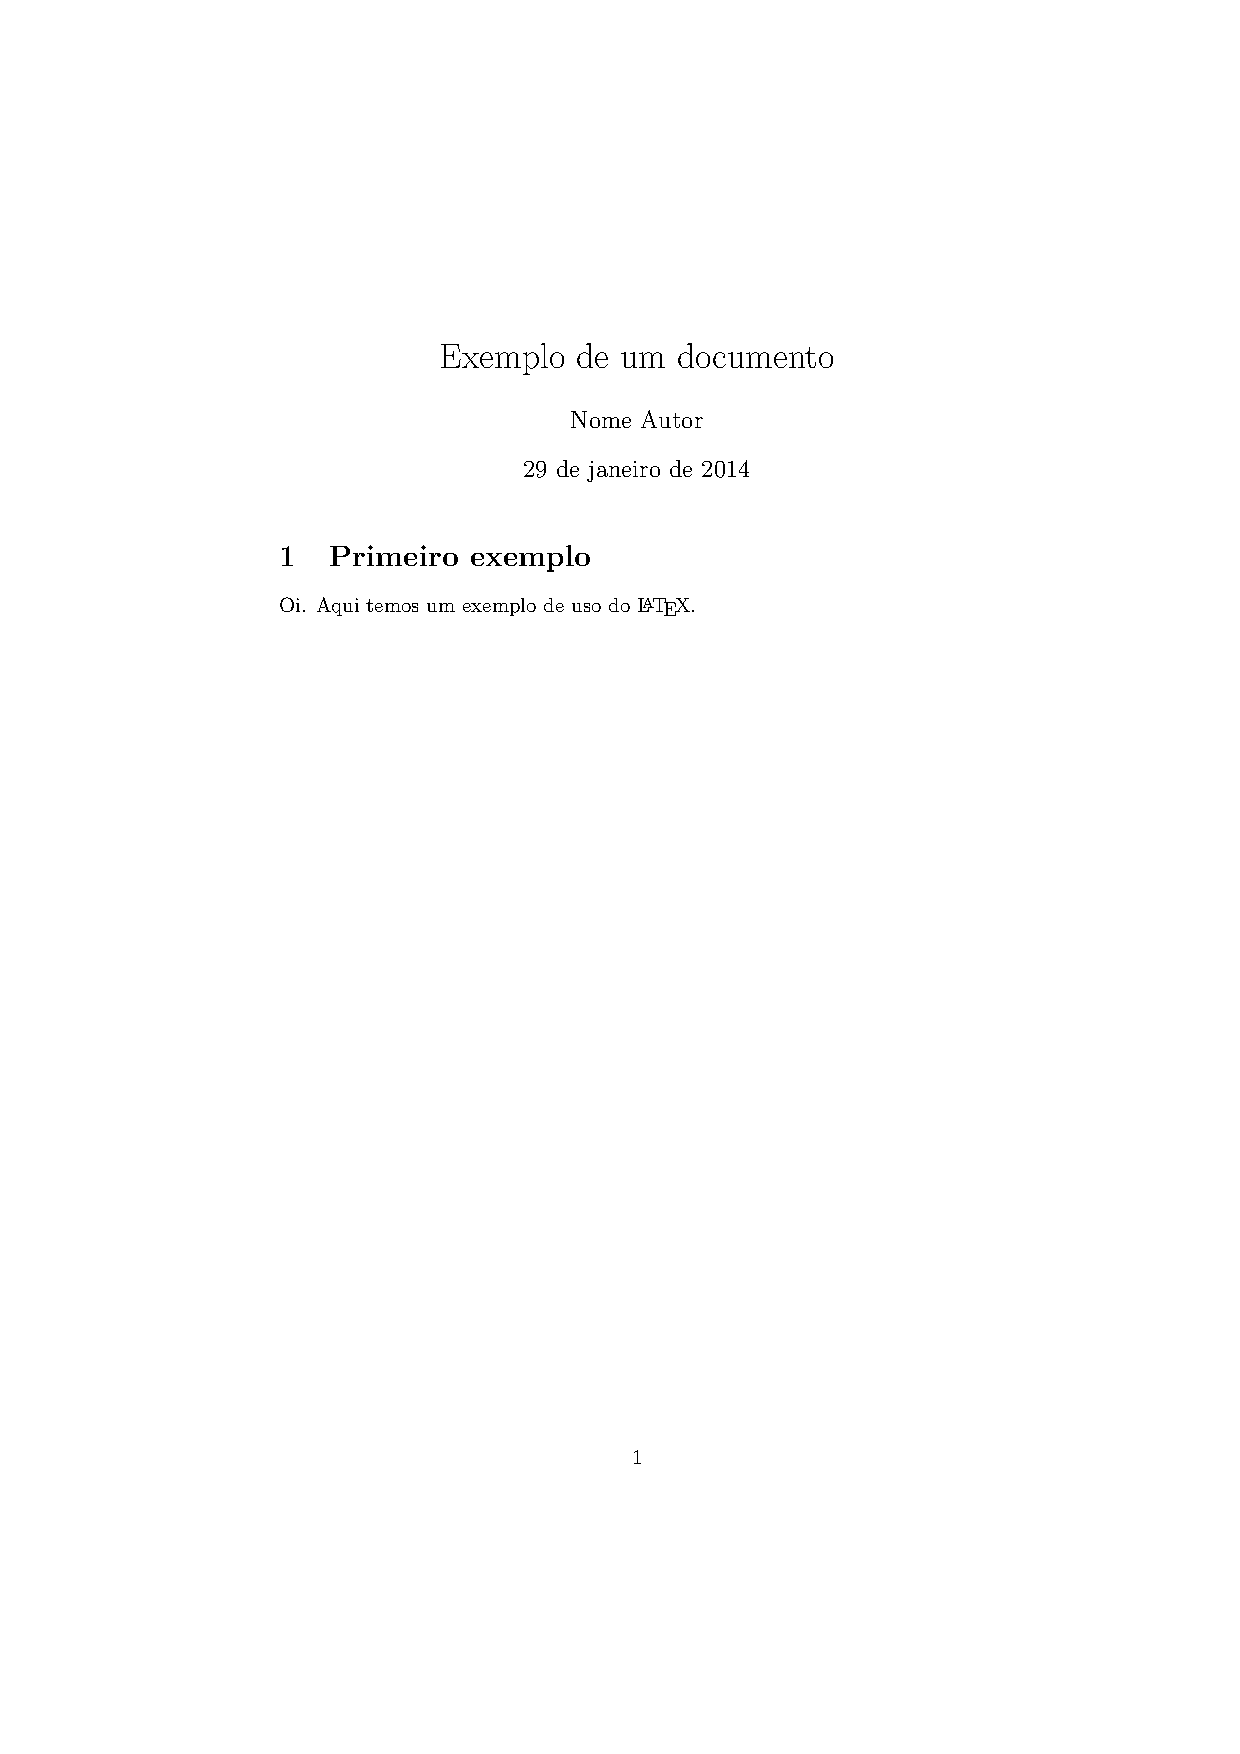
\includegraphics[trim= 0 18cm 0 5cm,clip]{conteudo/exemplo}}

Observe como, no código apresentado, não há nenhuma informação sobre que tipo de fonte utilizar, tamanho da letra, espaçamento entre linhas, posicionamento do título, etc. Estes detalhes são tratados pelo \LaTeX\ e o usuário não precisa se preocupar com eles. %TeX ao resgate!

\input{contents/inst} %Básicos da instalação

\input{contents/pratica} %Parte prática:

\bibliography{contents/handout_latex_2013-2}

\end{document}
